\documentclass[12pt,a4paper]{paper}
\usepackage[utf8]{inputenc}
\usepackage[english]{babel}
\usepackage{amsmath}
\usepackage{enumitem}
\usepackage{amsfonts}
\usepackage{amssymb}
\usepackage{amsmath}
\usepackage{tikz}
\usepackage{mathdots}
\usepackage{yhmath}
\usepackage{cancel}
\usepackage{color}
\usepackage{siunitx}
\usepackage{array}
\usepackage{multirow}
\usepackage{amssymb}
\usepackage{gensymb}
\usepackage{tabularx}
\usepackage{booktabs}
\usetikzlibrary{fadings}
\usepackage[left=2cm,right=2cm,top=2cm,bottom=2cm]{geometry}
\usepackage{Sweave}
\begin{document}
\title{STAT646 - Homework 4\\\small{Daniel Osorio - dcosorioh@tamu.edu\\Department of Veterinary Integrative Biosciences\\Texas A\&M University}}
\maketitle
\Sconcordance{concordance:Osorio_Daniel_HW4.tex:Osorio_Daniel_HW4.Rnw:%
1 22 1 1 0 15 1 1 2 1 0 1 2 4 0 1 2 50 1}

\begin{enumerate}
\item Use seqinr to obtain the human Genbank DNA sequence for the PSEN1 gene.
\begin{Schunk}
\begin{Sinput}
> library(seqinr)
> choosebank("genbank")
> hsaPSEN1 <- query(listname="PSEN1", query="SP=Homo sapiens AND K=PSEN1")
\end{Sinput}
\end{Schunk}
\begin{enumerate}
\item How many sequences are returned, what are they named, and what are their lengths?
\begin{Schunk}
\begin{Sinput}
> seqInfo <- lapply(hsaPSEN1$req, function(X){
+   c(X[1], attributes(X)[1])})
> seqInfo <- do.call(rbind.data.frame,seqInfo)
> colnames(seqInfo) <- c("seqName", "seqLength")
> rownames(seqInfo) <- NULL
> seqInfo
\end{Sinput}
\begin{Soutput}
          seqName seqLength
1        AB159776       142
2  AF416717.PSEN1      1137
3  BC011729.PSEN1      1392
4  KT120062.PSEN1      1404
5  KT120063.PSEN1      1404
6  KT120064.PSEN1      1404
7  KT120065.PSEN1      1404
8  KT120066.PSEN1      1404
9  KT120067.PSEN1      1404
10 KT599439.PSEN1      1404
11 KT599440.PSEN1      1404
12       KU178285      1389
13       KU178286      1401
14 KU178287.PSEN1       108
\end{Soutput}
\end{Schunk}
\item Provide the FASTA file entry for the first sequence (AB159776)
\begin{Schunk}
\begin{Sinput}
> id <- paste0(">", hsaPSEN1$req[[1]][1])
> seq <- toupper(unlist(getSequence(hsaPSEN1$req[1])))
> seq <- paste0(seq,collapse = "")
> seq <- unlist(strsplit(seq, "(?<=.{60})", perl = TRUE))
> writeLines(c(id,seq))
\end{Sinput}
\begin{Soutput}
>AB159776
AATCTATACCCCATTCACAGAAGATACCGAGACTGTGGGCCAGAGAGCCCTGCACTCAAT
TCTGAATGCTGCCATCATGATCAGTGTCATTGTTGTCATGACTATCCTCCTGGTGGTTCT
GAATAAATACAGGTGCTATAAG
\end{Soutput}
\end{Schunk}
\item What percentage of the bases in the third sequence (BC011729.PSEN1) are either G’s or C’s?
\begin{Schunk}
\begin{Sinput}
> seq <- toupper(unlist(getSequence(hsaPSEN1$req[3])))
> (sum(table(seq)[c("C","G")])/length(seq))*100
\end{Sinput}
\begin{Soutput}
[1] 46.12069
\end{Soutput}
\end{Schunk}
\end{enumerate}
\item Consider the global alignment of these two DNA sequences: GAG and GTAG. Let the score for a match be +1, the score for a mismatch be -1, and the score for a gap be -2 (so, opening a gap costs -2 points, extending that gap by one space costs an additional -2 points, and so on).
\begin{enumerate}
\item Write down the score matrix for this alignment, and fill in all of the cells. Your matrix should resemble that on slide 16 of the “alignment.pdf” slides under Notes on eCampus.
\begin{Schunk}
\begin{Soutput}
      G  T  A  G
   0 -2 -4 -6 -8
G -2  1 -1 -3 -5
A -4 -1  0  0 -2
G -6 -3 -2 -1  1
\end{Soutput}
\end{Schunk}
\item What is the optimal alignment, and what is its corresponding score?
\begin{Schunk}
\begin{Sinput}
> library(Biostrings)
> pMatrix <- nucleotideSubstitutionMatrix(match = 1, mismatch = -1)
> pairwiseAlignment(pattern = "GAG",subject = "GTAG", 
+                   substitutionMatrix = pMatrix, 
+                   gapOpening = -2, gapExtension = -2)
\end{Sinput}
\begin{Soutput}
Global PairwiseAlignmentsSingleSubject (1 of 1)
pattern: G-AG
subject: GTAG
score: -1 
\end{Soutput}
\end{Schunk}
\end{enumerate}
\item Consider these two amino acid sequences: ASEDLTI and AEEDFGI. For the purposes of alignment, use the PAM30 error matrix and a gap penalty of -2 (gap open =0 and gap extend = -2).
\begin{enumerate}
\item What are the optimal alignments, using both the global and local algorithms?
\begin{Schunk}
\begin{Sinput}
> pairwiseAlignment(pattern = "ASEDLTI", subject = "AEEDFGI",
+                   substitutionMatrix = 'PAM30', gapOpening = 0, 
+                   gapExtension = -2, type = "local")
\end{Sinput}
\begin{Soutput}
Local PairwiseAlignmentsSingleSubject (1 of 1)
pattern: [1] ASEDL-TI
subject: [1] AEEDFG-I
score: 19 
\end{Soutput}
\begin{Sinput}
> pairwiseAlignment(pattern = "ASEDLTI", subject = "AEEDFGI",
+                   substitutionMatrix = 'PAM30', gapOpening = 0, 
+                   gapExtension = -2, type = "global")
\end{Sinput}
\begin{Soutput}
Global PairwiseAlignmentsSingleSubject (1 of 1)
pattern: ASEDL-TI
subject: AEEDFG-I
score: 19 
\end{Soutput}
\end{Schunk}
\item Verify the overall scores for these alignments.
\item Use the randomization-based significance test we used in class to assess the local alignment of the two amino acid sequences:
\begin{enumerate}
\item Report a density plot of the randomization based alignment scores; use the den- sity function. Shade in the area under the density curve that corresponds to the randomization based scores that are $\ge$ our observed score of 19.
\item What is the resulting p-value?
\end{enumerate}
\end{enumerate}
\item The H1F0 gene is present in multiple species. The versions of the gene in human, mouse, and cow are said to be homologous.
\begin{Schunk}
\begin{Sinput}
> humanH1F0 <- query(listname = "H1F0", query = "SP=Homo sapiens AND K=H1F0")
> humanH1F0 <- unlist(getSequence(humanH1F0$req[1]))
> mouseH1F0 <- query(listname = "H1F0", query = "SP=Mus musculus AND K=H1F0")
> mouseH1F0 <- unlist(getSequence(mouseH1F0$req[1]))
> cowH1F0 <- query(listname = "H1F0", query = "SP=Bos taurus AND K=H1F0")
> cowH1F0 <- unlist(getSequence(cowH1F0$req[1]))
\end{Sinput}
\end{Schunk}
\begin{enumerate}
\item What does homologous mean?
\textit{Homologous means similar in position, structure, and evolutionary origin but not necessarily in function.}
\item Consider the global alignment of the sequences of this gene in human (homo sapiens) and mouse (mus musculus). Use seqinr to download the DNA sequences. You will get multiple sequences for each species. Just use the first of each. The lengths of the human and mouse sequences will be the same. [ Use gap open = 0 and gap extend = -2]
\begin{enumerate}
\item Comparing the human and mouse versions of H1F0, what proportion of bases differ?
\begin{Schunk}
\begin{Sinput}
> mean(humanH1F0 != mouseH1F0)
\end{Sinput}
\begin{Soutput}
[1] 0.08888889
\end{Soutput}
\end{Schunk}
\item Report a dot plot showing their alignment.
\begin{Schunk}
\begin{Sinput}
> par(mar=c(2.5,2.5,1,1), mgp=c(1.5,0.5,0))
> dotPlot(humanH1F0,cowH1F0)
\end{Sinput}
\end{Schunk}
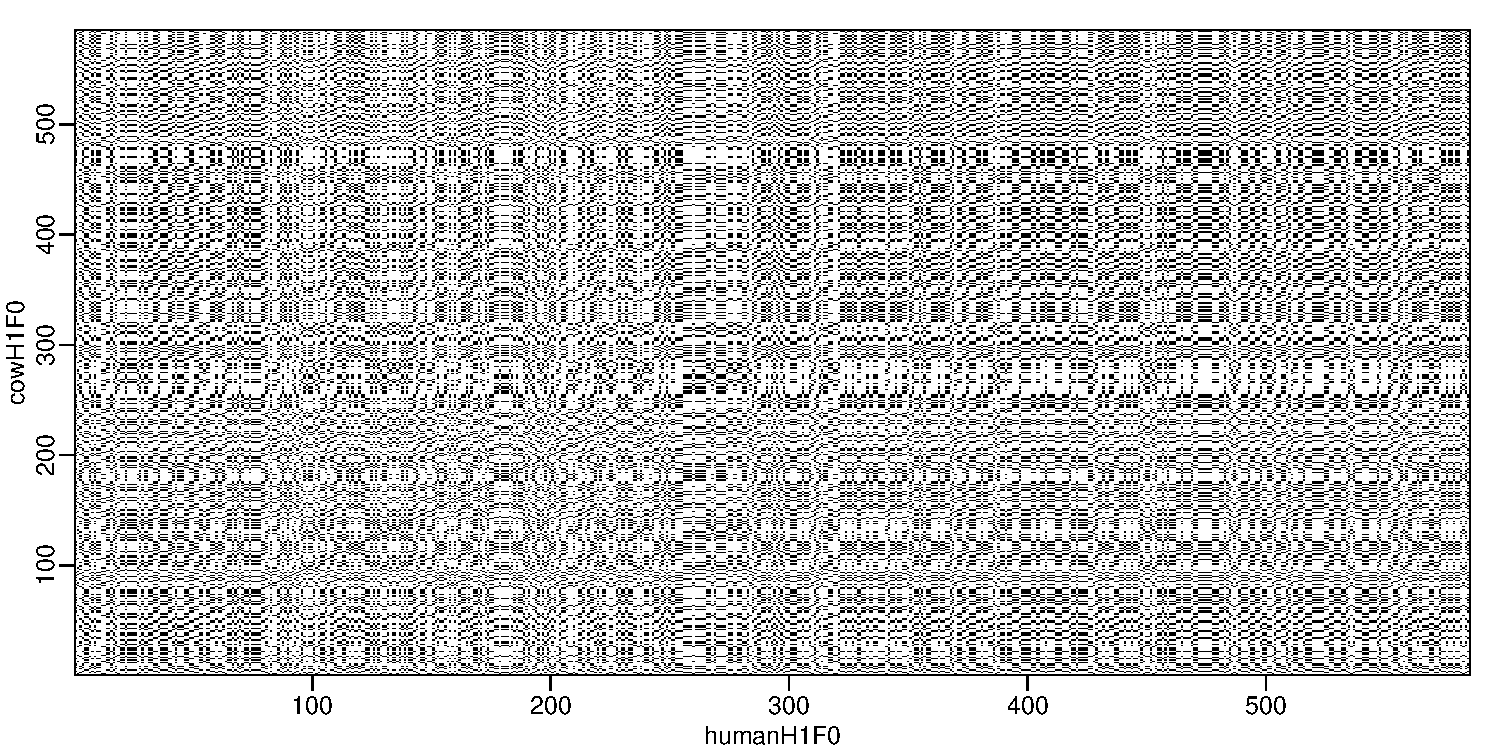
\includegraphics{Osorio_Daniel_HW4-010}
\item Use the randomization-based significance test to assess the global alignment of H1F0 in human and mouse. What is the p-value?[ Use gap open = 0 and gap extend = -2]
\end{enumerate}
\item Use the muscle package to carry out multiple alignment of H1F0 in human, mouse, and cow (bos taurus). Again, just use the first sequence returned by seqinr for each species. Report the first 50 aligned bases.
\begin{Schunk}
\begin{Sinput}
> library(muscle)
> humanH1F0 <- paste0(humanH1F0[1:50], collapse = "")
> mouseH1F0 <- paste0(mouseH1F0[1:50], collapse = "")
> cowH1F0 <- paste0(cowH1F0[1:50], collapse = "")
> H1F0 <- DNAStringSet(c(humanH1F0,mouseH1F0,cowH1F0))
> muscle(H1F0)
\end{Sinput}
\begin{Soutput}
MUSCLE v3.8.31 by Robert C. Edgar

http://www.drive5.com/muscle
This software is donated to the public domain.
Please cite: Edgar, R.C. Nucleic Acids Res 32(5), 1792-97.

file1e767bcea0b 3 seqs, max length 50, avg  length 50
138 MB(3%)00:00:00                Iter   1   16.67%  K-mer dist pass 1
138 MB(3%)00:00:00                Iter   1  100.00%  K-mer dist pass 1
138 MB(3%)00:00:00                Iter   1   16.67%  K-mer dist pass 2
138 MB(3%)00:00:00                Iter   1  100.00%  K-mer dist pass 2
138 MB(3%)00:00:00                Iter   1   50.00%  Align node       
139 MB(3%)00:00:00                Iter   1  100.00%  Align node
139 MB(3%)00:00:00                Iter   1  100.00%  Align node
139 MB(3%)00:00:00                Iter   1   33.33%  Root alignment
139 MB(3%)00:00:00                Iter   1   66.67%  Root alignment
139 MB(3%)00:00:00                Iter   1  100.00%  Root alignment
139 MB(3%)00:00:00                Iter   1  100.00%  Root alignment
139 MB(3%)00:00:00                Iter   2  100.00%  Root alignment
139 MB(3%)00:00:00                Iter   3   66.67%  Refine biparts
139 MB(3%)00:00:00                Iter   3  100.00%  Refine biparts
139 MB(3%)00:00:00                Iter   3  133.33%  Refine biparts
139 MB(3%)00:00:00                Iter   3  100.00%  Refine biparts
DNAMultipleAlignment with 3 rows and 50 columns
     aln
[1] ATGACCGAGAATTCCACGTCCGCCCCTGCGGCCAAGCCCAAGCGGGCCAA
[2] ATGACCGAGAACTCCACCTCCGCCCCGGCGGCGAAGCCCAAACGGGCCAA
[3] ATGACCGAGAACTCCACGTCCACCCCTGCGGCCAAGCCCAAGCGGGCCAA
\end{Soutput}
\end{Schunk}
\end{enumerate}
\item Download the “QC spike” data from eCampus. These are mass spectrometry proteomics data. There are 12 samples. In each sample, there is mostly Salmonella proteins, but a small number of “quality control” (QC) proteins are spiked in as well. The first four samples are replicates for which the QC proteins were spiked at a high concentration, the next four samples have QC proteins at a medium concentration, and the last four samples have QC proteins at a low concentration. The numeric values in the data are quantifications of the prevalences of 4,591 peptides in each sample (larger numbers mean more copies of the corresponding peptide). The first column is a unique identifier for each peptide. The next few columns provide additional information about the peptides and the proteins they correspond to. The column named “is qc” is an indicator for whether each peptide came from a QC protein (1 if yes, 0 if no). The remaining 12 columns contain the peptide intensities themselves.
\begin{Schunk}
\begin{Sinput}
> qcData <- read.csv("qc_spike.csv")
\end{Sinput}
\end{Schunk}
\begin{enumerate}
\item Filter out all peptides for which at least one comparison group has fewer than 2 observations (non-NA values). After completing this, you should be left only with peptides for which each comparison group has at least 2 observations. How many peptides are you left with? How many of these are QC peptides, and how many are Salmonella peptides? Use these filtered data in what follows.
\begin{Schunk}
\begin{Sinput}
> g0 <- grepl("G0",colnames(qcData))
> g1 <- grepl("G1",colnames(qcData))
> g2 <- grepl("G2",colnames(qcData))
> sPeptides <- apply(qcData, 1, function(X){
+   sum(is.na(X[g0])) <= 2 & 
+   sum(is.na(X[g2])) <= 2 & 
+   sum(is.na(X[g1])) <= 2
+ })
> qcData <- qcData[sPeptides,]
> table(qcData$is_qc)
\end{Sinput}
\begin{Soutput}
   0    1 
1703   30 
\end{Soutput}
\end{Schunk}
\item Report side-by-side boxplots comparing the 12 samples (so, 12 boxplots side-by-side), for the QC peptides.
\begin{Schunk}
\begin{Sinput}
> par(mar=c(2.5,2.5,1,1), mgp=c(1.5,0.5,0))
> boxplot(qcData[qcData$is_qc == 1,8:19])
\end{Sinput}
\end{Schunk}
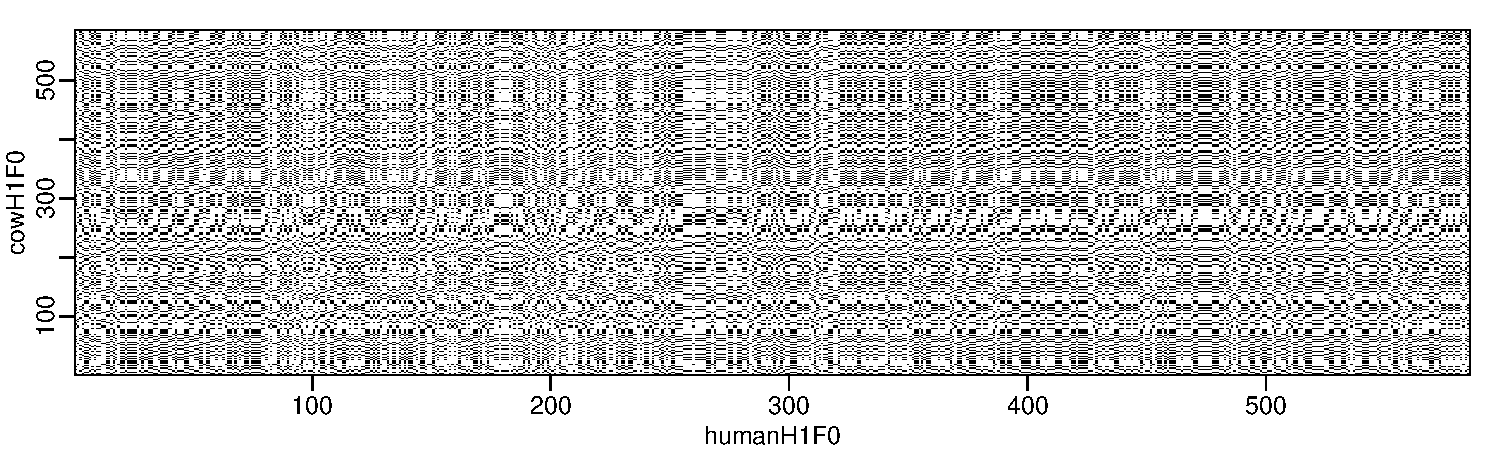
\includegraphics{Osorio_Daniel_HW4-014}
\item Report side-by-side boxplots comparing the 12 samples, now for the Salmonella peptides.
\begin{Schunk}
\begin{Sinput}
> par(mar=c(2.5,2.5,1,1), mgp=c(1.5,0.5,0))
> boxplot(qcData[qcData$is_qc == 0,8:19])
\end{Sinput}
\end{Schunk}
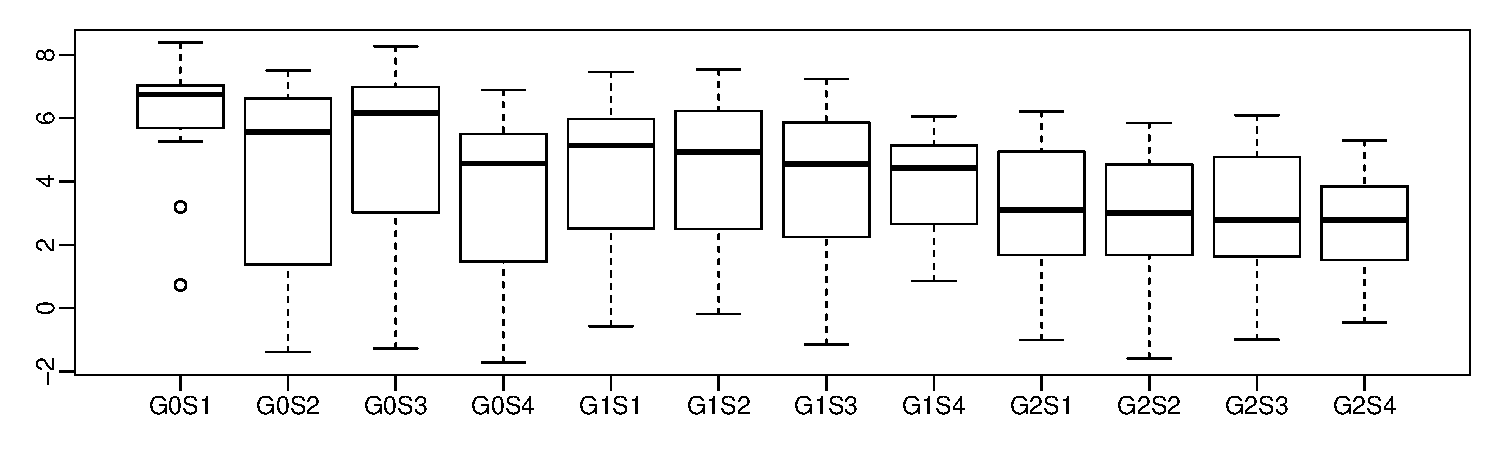
\includegraphics{Osorio_Daniel_HW4-015}
\item For each of the Salmonella peptides, compute a two-sample t-test, assuming equal variances, comparing the first comparison group (highest concentration of QC proteins) to the third comparison group (lowest concentration of QC proteins).
\begin{Schunk}
\begin{Sinput}
> pValues <- apply(qcData[qcData$is_qc == 0,], 1, function(X){
+   t.test(as.numeric(X[g0]),as.numeric(X[g2]),var.equal = TRUE)$p.value
+ })
\end{Sinput}
\end{Schunk}
\begin{enumerate}
\item Report a histogram of the resulting p-values.
\begin{Schunk}
\begin{Sinput}
> par(mar=c(2.5,2.5,1,1), mgp=c(1.5,0.5,0))
> hist(pValues, probability = TRUE,breaks = 20, main = "P Values")
> abline(v=0.05, lty=2, col="red", lwd = 2)
\end{Sinput}
\end{Schunk}
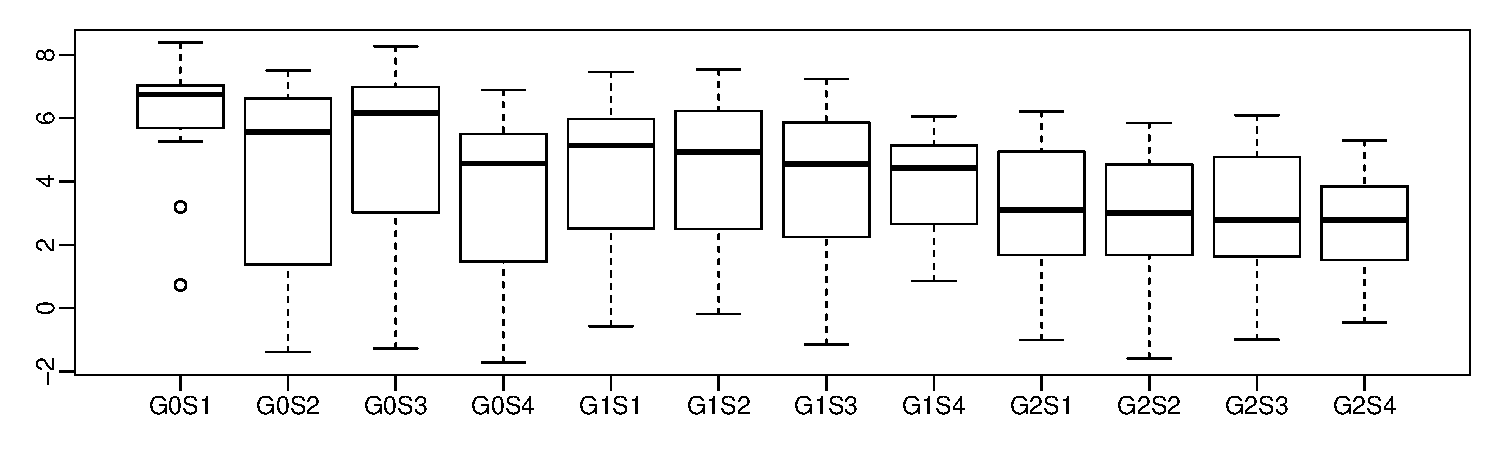
\includegraphics{Osorio_Daniel_HW4-017}
\item What proportion of the Salmonella peptides had p-values < 0.05? What proportion
of the Salmonella peptides did you expect to have p-values < 0.05? \textit{By chance I expect to have 5\% of p-values < 0.05}
\begin{Schunk}
\begin{Sinput}
> mean(pValues < 0.05)
\end{Sinput}
\begin{Soutput}
[1] 0.1280094
\end{Soutput}
\end{Schunk}
\end{enumerate}
\end{enumerate}
\end{enumerate}
\end{document}
